\documentclass[11pt,]{article}
\usepackage[left=0.5in,top=0.75in,right=0.3in,bottom=0.3in]{geometry}
\newcommand*{\authorfont}{\fontfamily{phv}\selectfont}
\usepackage[]{mathpazo}


  \usepackage[T1]{fontenc}
  \usepackage[utf8]{inputenc}



\usepackage{abstract}
\renewcommand{\abstractname}{}    % clear the title
\renewcommand{\absnamepos}{empty} % originally center

\renewenvironment{abstract}
 {{%
    \setlength{\leftmargin}{0mm}
    \setlength{\rightmargin}{\leftmargin}%
  }%
  \relax}
 {\endlist}

\makeatletter
\def\@maketitle{%
  \newpage
%  \null
%  \vskip 2em%
%  \begin{center}%
  \let \footnote \thanks
    {\fontsize{18}{20}\selectfont\raggedright  \setlength{\parindent}{0pt} \@title \par}%
}
%\fi
\makeatother




\setcounter{secnumdepth}{0}

\usepackage{color}
\usepackage{fancyvrb}
\newcommand{\VerbBar}{|}
\newcommand{\VERB}{\Verb[commandchars=\\\{\}]}
\DefineVerbatimEnvironment{Highlighting}{Verbatim}{commandchars=\\\{\}}
% Add ',fontsize=\small' for more characters per line
\usepackage{framed}
\definecolor{shadecolor}{RGB}{248,248,248}
\newenvironment{Shaded}{\begin{snugshade}}{\end{snugshade}}
\newcommand{\AlertTok}[1]{\textcolor[rgb]{0.94,0.16,0.16}{#1}}
\newcommand{\AnnotationTok}[1]{\textcolor[rgb]{0.56,0.35,0.01}{\textbf{\textit{#1}}}}
\newcommand{\AttributeTok}[1]{\textcolor[rgb]{0.77,0.63,0.00}{#1}}
\newcommand{\BaseNTok}[1]{\textcolor[rgb]{0.00,0.00,0.81}{#1}}
\newcommand{\BuiltInTok}[1]{#1}
\newcommand{\CharTok}[1]{\textcolor[rgb]{0.31,0.60,0.02}{#1}}
\newcommand{\CommentTok}[1]{\textcolor[rgb]{0.56,0.35,0.01}{\textit{#1}}}
\newcommand{\CommentVarTok}[1]{\textcolor[rgb]{0.56,0.35,0.01}{\textbf{\textit{#1}}}}
\newcommand{\ConstantTok}[1]{\textcolor[rgb]{0.00,0.00,0.00}{#1}}
\newcommand{\ControlFlowTok}[1]{\textcolor[rgb]{0.13,0.29,0.53}{\textbf{#1}}}
\newcommand{\DataTypeTok}[1]{\textcolor[rgb]{0.13,0.29,0.53}{#1}}
\newcommand{\DecValTok}[1]{\textcolor[rgb]{0.00,0.00,0.81}{#1}}
\newcommand{\DocumentationTok}[1]{\textcolor[rgb]{0.56,0.35,0.01}{\textbf{\textit{#1}}}}
\newcommand{\ErrorTok}[1]{\textcolor[rgb]{0.64,0.00,0.00}{\textbf{#1}}}
\newcommand{\ExtensionTok}[1]{#1}
\newcommand{\FloatTok}[1]{\textcolor[rgb]{0.00,0.00,0.81}{#1}}
\newcommand{\FunctionTok}[1]{\textcolor[rgb]{0.00,0.00,0.00}{#1}}
\newcommand{\ImportTok}[1]{#1}
\newcommand{\InformationTok}[1]{\textcolor[rgb]{0.56,0.35,0.01}{\textbf{\textit{#1}}}}
\newcommand{\KeywordTok}[1]{\textcolor[rgb]{0.13,0.29,0.53}{\textbf{#1}}}
\newcommand{\NormalTok}[1]{#1}
\newcommand{\OperatorTok}[1]{\textcolor[rgb]{0.81,0.36,0.00}{\textbf{#1}}}
\newcommand{\OtherTok}[1]{\textcolor[rgb]{0.56,0.35,0.01}{#1}}
\newcommand{\PreprocessorTok}[1]{\textcolor[rgb]{0.56,0.35,0.01}{\textit{#1}}}
\newcommand{\RegionMarkerTok}[1]{#1}
\newcommand{\SpecialCharTok}[1]{\textcolor[rgb]{0.00,0.00,0.00}{#1}}
\newcommand{\SpecialStringTok}[1]{\textcolor[rgb]{0.31,0.60,0.02}{#1}}
\newcommand{\StringTok}[1]{\textcolor[rgb]{0.31,0.60,0.02}{#1}}
\newcommand{\VariableTok}[1]{\textcolor[rgb]{0.00,0.00,0.00}{#1}}
\newcommand{\VerbatimStringTok}[1]{\textcolor[rgb]{0.31,0.60,0.02}{#1}}
\newcommand{\WarningTok}[1]{\textcolor[rgb]{0.56,0.35,0.01}{\textbf{\textit{#1}}}}
\usepackage{longtable,booktabs}

\usepackage{graphicx,grffile}
\makeatletter
\def\maxwidth{\ifdim\Gin@nat@width>\linewidth\linewidth\else\Gin@nat@width\fi}
\def\maxheight{\ifdim\Gin@nat@height>\textheight\textheight\else\Gin@nat@height\fi}
\makeatother
% Scale images if necessary, so that they will not overflow the page
% margins by default, and it is still possible to overwrite the defaults
% using explicit options in \includegraphics[width, height, ...]{}
\setkeys{Gin}{width=\maxwidth,height=\maxheight,keepaspectratio}

\title{Lab 5 Two factor Factorial 1  }



\author{\Large Shen Qu\vspace{0.05in} \newline\normalsize\emph{March 09, 2019}  }


\date{}

\usepackage{titlesec}

\titleformat*{\section}{\normalsize\bfseries}
\titleformat*{\subsection}{\normalsize\itshape}
\titleformat*{\subsubsection}{\normalsize\itshape}
\titleformat*{\paragraph}{\normalsize\itshape}
\titleformat*{\subparagraph}{\normalsize\itshape}


\usepackage{natbib}
\bibliographystyle{plainnat}
\usepackage[strings]{underscore} % protect underscores in most circumstances



\newtheorem{hypothesis}{Hypothesis}
\usepackage{setspace}

\makeatletter
\@ifpackageloaded{hyperref}{}{%
\ifxetex
  \PassOptionsToPackage{hyphens}{url}\usepackage[setpagesize=false, % page size defined by xetex
              unicode=false, % unicode breaks when used with xetex
              xetex]{hyperref}
\else
  \PassOptionsToPackage{hyphens}{url}\usepackage[unicode=true]{hyperref}
\fi
}

\@ifpackageloaded{color}{
    \PassOptionsToPackage{usenames,dvipsnames}{color}
}{%
    \usepackage[usenames,dvipsnames]{color}
}
\makeatother
\hypersetup{breaklinks=true,
            bookmarks=true,
            pdfauthor={Shen Qu (March 09, 2019)},
             pdfkeywords = {},  
            pdftitle={Lab 5 Two factor Factorial 1},
            colorlinks=true,
            citecolor=blue,
            urlcolor=blue,
            linkcolor=magenta,
            pdfborder={0 0 0}}
\urlstyle{same}  % don't use monospace font for urls

% set default figure placement to htbp
\makeatletter
\def\fps@figure{htbp}
\makeatother



% add tightlist ----------
\providecommand{\tightlist}{%
\setlength{\itemsep}{0pt}\setlength{\parskip}{0pt}}

\begin{document}
	
% \pagenumbering{arabic}% resets `page` counter to 1 
%
% \maketitle

{% \usefont{T1}{pnc}{m}{n}
\setlength{\parindent}{0pt}
\thispagestyle{plain}
{\fontsize{18}{20}\selectfont\raggedright 
\maketitle  % title \par  

}

{
   \vskip 13.5pt\relax \normalsize\fontsize{11}{12} 
\textbf{\authorfont Shen Qu} \hskip 15pt \emph{\small March 09, 2019}   

}

}








\begin{abstract}

    \hbox{\vrule height .2pt width 39.14pc}

    \vskip 8.5pt % \small 

\noindent An experiment was designed to study weight gain of rats fed four
different diets, where there were two levels of protein (high or low)
and two sources of protein (beef or cereal). This gives 2 x 2 treatment
combinations: high/beef (HB), high/cereal (HC), low/beef (LB),
low/cereal (LC). Ten rats were in each of the four treatment groups. Use
a=0.01


    \hbox{\vrule height .2pt width 39.14pc}


\end{abstract}


\vskip 6.5pt


\noindent  (a).
\textcolor[rgb]{0.5,0.5,0.5}{Plot the data and report the plot here (A plot with data and means of treatment combinations). Do not report code here. Describe the observed relationship between two factors.}

\begin{verbatim}
## Observations: 40
## Variables: 5
## $ Source <chr> "Beef", "Beef", "Beef", "Beef", "Beef", "Beef", "Beef",...
## $ Amount <chr> "Low", "Low", "Low", "Low", "Low", "Low", "Low", "Low",...
## $ Gain   <dbl> 90, 76, 90, 64, 86, 51, 72, 90, 95, 78, 73, 102, 118, 1...
## $ Trt1   <fct> Beef, Beef, Beef, Beef, Beef, Beef, Beef, Beef, Beef, B...
## $ Trt2   <fct> Low, Low, Low, Low, Low, Low, Low, Low, Low, Low, High,...
\end{verbatim}

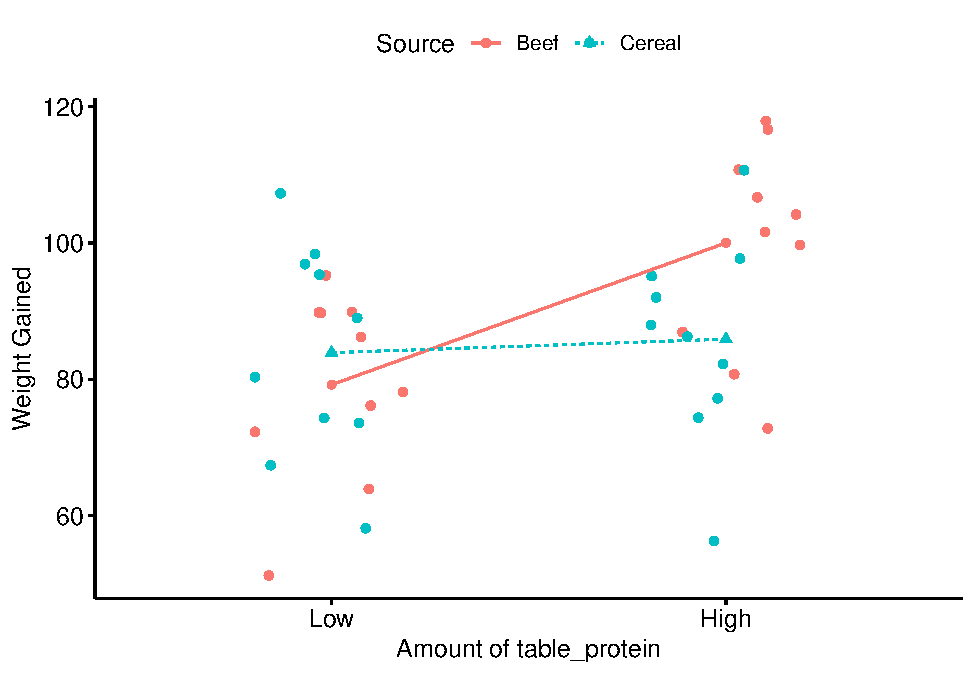
\includegraphics{svm-rmarkdown-article-example_files/figure-latex/unnamed-chunk-3-1.pdf}

(b).
\textcolor[rgb]{0.5,0.5,0.5}{Obtain the numerical summary for each treatment combination and factor levels separately. Report them here in a tabular form.}

\begin{longtable}[]{@{}cccccccccc@{}}
\toprule
\begin{minipage}[b]{0.09\columnwidth}\centering
Source\strut
\end{minipage} & \begin{minipage}[b]{0.06\columnwidth}\centering
min\strut
\end{minipage} & \begin{minipage}[b]{0.07\columnwidth}\centering
Q1\strut
\end{minipage} & \begin{minipage}[b]{0.09\columnwidth}\centering
median\strut
\end{minipage} & \begin{minipage}[b]{0.08\columnwidth}\centering
Q3\strut
\end{minipage} & \begin{minipage}[b]{0.06\columnwidth}\centering
max\strut
\end{minipage} & \begin{minipage}[b]{0.07\columnwidth}\centering
mean\strut
\end{minipage} & \begin{minipage}[b]{0.08\columnwidth}\centering
sd\strut
\end{minipage} & \begin{minipage}[b]{0.05\columnwidth}\centering
n\strut
\end{minipage} & \begin{minipage}[b]{0.10\columnwidth}\centering
missing\strut
\end{minipage}\tabularnewline
\midrule
\endhead
\begin{minipage}[t]{0.09\columnwidth}\centering
Beef\strut
\end{minipage} & \begin{minipage}[t]{0.06\columnwidth}\centering
51\strut
\end{minipage} & \begin{minipage}[t]{0.07\columnwidth}\centering
77.5\strut
\end{minipage} & \begin{minipage}[t]{0.09\columnwidth}\centering
90\strut
\end{minipage} & \begin{minipage}[t]{0.08\columnwidth}\centering
102.5\strut
\end{minipage} & \begin{minipage}[t]{0.06\columnwidth}\centering
118\strut
\end{minipage} & \begin{minipage}[t]{0.07\columnwidth}\centering
89.6\strut
\end{minipage} & \begin{minipage}[t]{0.08\columnwidth}\centering
17.71\strut
\end{minipage} & \begin{minipage}[t]{0.05\columnwidth}\centering
20\strut
\end{minipage} & \begin{minipage}[t]{0.10\columnwidth}\centering
0\strut
\end{minipage}\tabularnewline
\begin{minipage}[t]{0.09\columnwidth}\centering
Cereal\strut
\end{minipage} & \begin{minipage}[t]{0.06\columnwidth}\centering
56\strut
\end{minipage} & \begin{minipage}[t]{0.07\columnwidth}\centering
74\strut
\end{minipage} & \begin{minipage}[t]{0.09\columnwidth}\centering
87\strut
\end{minipage} & \begin{minipage}[t]{0.08\columnwidth}\centering
95.5\strut
\end{minipage} & \begin{minipage}[t]{0.06\columnwidth}\centering
111\strut
\end{minipage} & \begin{minipage}[t]{0.07\columnwidth}\centering
84.9\strut
\end{minipage} & \begin{minipage}[t]{0.08\columnwidth}\centering
14.99\strut
\end{minipage} & \begin{minipage}[t]{0.05\columnwidth}\centering
20\strut
\end{minipage} & \begin{minipage}[t]{0.10\columnwidth}\centering
0\strut
\end{minipage}\tabularnewline
\bottomrule
\end{longtable}

\begin{longtable}[]{@{}cccccccccc@{}}
\toprule
\begin{minipage}[b]{0.13\columnwidth}\centering
Amount\strut
\end{minipage} & \begin{minipage}[b]{0.05\columnwidth}\centering
min\strut
\end{minipage} & \begin{minipage}[b]{0.07\columnwidth}\centering
Q1\strut
\end{minipage} & \begin{minipage}[b]{0.08\columnwidth}\centering
median\strut
\end{minipage} & \begin{minipage}[b]{0.07\columnwidth}\centering
Q3\strut
\end{minipage} & \begin{minipage}[b]{0.05\columnwidth}\centering
max\strut
\end{minipage} & \begin{minipage}[b]{0.07\columnwidth}\centering
mean\strut
\end{minipage} & \begin{minipage}[b]{0.07\columnwidth}\centering
sd\strut
\end{minipage} & \begin{minipage}[b]{0.04\columnwidth}\centering
n\strut
\end{minipage} & \begin{minipage}[b]{0.09\columnwidth}\centering
missing\strut
\end{minipage}\tabularnewline
\midrule
\endhead
\begin{minipage}[t]{0.13\columnwidth}\centering
Beef.High\strut
\end{minipage} & \begin{minipage}[t]{0.05\columnwidth}\centering
73\strut
\end{minipage} & \begin{minipage}[t]{0.07\columnwidth}\centering
90.25\strut
\end{minipage} & \begin{minipage}[t]{0.08\columnwidth}\centering
103\strut
\end{minipage} & \begin{minipage}[t]{0.07\columnwidth}\centering
110\strut
\end{minipage} & \begin{minipage}[t]{0.05\columnwidth}\centering
118\strut
\end{minipage} & \begin{minipage}[t]{0.07\columnwidth}\centering
100\strut
\end{minipage} & \begin{minipage}[t]{0.07\columnwidth}\centering
15.14\strut
\end{minipage} & \begin{minipage}[t]{0.04\columnwidth}\centering
10\strut
\end{minipage} & \begin{minipage}[t]{0.09\columnwidth}\centering
0\strut
\end{minipage}\tabularnewline
\begin{minipage}[t]{0.13\columnwidth}\centering
Cereal.High\strut
\end{minipage} & \begin{minipage}[t]{0.05\columnwidth}\centering
56\strut
\end{minipage} & \begin{minipage}[t]{0.07\columnwidth}\centering
78.25\strut
\end{minipage} & \begin{minipage}[t]{0.08\columnwidth}\centering
87\strut
\end{minipage} & \begin{minipage}[t]{0.07\columnwidth}\centering
94.25\strut
\end{minipage} & \begin{minipage}[t]{0.05\columnwidth}\centering
111\strut
\end{minipage} & \begin{minipage}[t]{0.07\columnwidth}\centering
85.9\strut
\end{minipage} & \begin{minipage}[t]{0.07\columnwidth}\centering
15.02\strut
\end{minipage} & \begin{minipage}[t]{0.04\columnwidth}\centering
10\strut
\end{minipage} & \begin{minipage}[t]{0.09\columnwidth}\centering
0\strut
\end{minipage}\tabularnewline
\begin{minipage}[t]{0.13\columnwidth}\centering
Beef.Low\strut
\end{minipage} & \begin{minipage}[t]{0.05\columnwidth}\centering
51\strut
\end{minipage} & \begin{minipage}[t]{0.07\columnwidth}\centering
73\strut
\end{minipage} & \begin{minipage}[t]{0.08\columnwidth}\centering
82\strut
\end{minipage} & \begin{minipage}[t]{0.07\columnwidth}\centering
90\strut
\end{minipage} & \begin{minipage}[t]{0.05\columnwidth}\centering
95\strut
\end{minipage} & \begin{minipage}[t]{0.07\columnwidth}\centering
79.2\strut
\end{minipage} & \begin{minipage}[t]{0.07\columnwidth}\centering
13.89\strut
\end{minipage} & \begin{minipage}[t]{0.04\columnwidth}\centering
10\strut
\end{minipage} & \begin{minipage}[t]{0.09\columnwidth}\centering
0\strut
\end{minipage}\tabularnewline
\begin{minipage}[t]{0.13\columnwidth}\centering
Cereal.Low\strut
\end{minipage} & \begin{minipage}[t]{0.05\columnwidth}\centering
58\strut
\end{minipage} & \begin{minipage}[t]{0.07\columnwidth}\centering
74\strut
\end{minipage} & \begin{minipage}[t]{0.08\columnwidth}\centering
84.5\strut
\end{minipage} & \begin{minipage}[t]{0.07\columnwidth}\centering
96.5\strut
\end{minipage} & \begin{minipage}[t]{0.05\columnwidth}\centering
107\strut
\end{minipage} & \begin{minipage}[t]{0.07\columnwidth}\centering
83.9\strut
\end{minipage} & \begin{minipage}[t]{0.07\columnwidth}\centering
15.71\strut
\end{minipage} & \begin{minipage}[t]{0.04\columnwidth}\centering
10\strut
\end{minipage} & \begin{minipage}[t]{0.09\columnwidth}\centering
0\strut
\end{minipage}\tabularnewline
\begin{minipage}[t]{0.13\columnwidth}\centering
High\strut
\end{minipage} & \begin{minipage}[t]{0.05\columnwidth}\centering
56\strut
\end{minipage} & \begin{minipage}[t]{0.07\columnwidth}\centering
81.75\strut
\end{minipage} & \begin{minipage}[t]{0.08\columnwidth}\centering
93.5\strut
\end{minipage} & \begin{minipage}[t]{0.07\columnwidth}\centering
104.8\strut
\end{minipage} & \begin{minipage}[t]{0.05\columnwidth}\centering
118\strut
\end{minipage} & \begin{minipage}[t]{0.07\columnwidth}\centering
92.95\strut
\end{minipage} & \begin{minipage}[t]{0.07\columnwidth}\centering
16.36\strut
\end{minipage} & \begin{minipage}[t]{0.04\columnwidth}\centering
20\strut
\end{minipage} & \begin{minipage}[t]{0.09\columnwidth}\centering
0\strut
\end{minipage}\tabularnewline
\begin{minipage}[t]{0.13\columnwidth}\centering
Low\strut
\end{minipage} & \begin{minipage}[t]{0.05\columnwidth}\centering
51\strut
\end{minipage} & \begin{minipage}[t]{0.07\columnwidth}\centering
73.5\strut
\end{minipage} & \begin{minipage}[t]{0.08\columnwidth}\centering
83\strut
\end{minipage} & \begin{minipage}[t]{0.07\columnwidth}\centering
91.25\strut
\end{minipage} & \begin{minipage}[t]{0.05\columnwidth}\centering
107\strut
\end{minipage} & \begin{minipage}[t]{0.07\columnwidth}\centering
81.55\strut
\end{minipage} & \begin{minipage}[t]{0.07\columnwidth}\centering
14.63\strut
\end{minipage} & \begin{minipage}[t]{0.04\columnwidth}\centering
20\strut
\end{minipage} & \begin{minipage}[t]{0.09\columnwidth}\centering
0\strut
\end{minipage}\tabularnewline
\bottomrule
\end{longtable}

(c).
\textcolor[rgb]{0.5,0.5,0.5}{Fit the two-factor factorial model and report the complete ANOVA table here. Do not report code here. The complete ANOVA table should have a row for each of the following: main effects of each treatment, two-factor interaction effects, error and total.}

\begin{verbatim}
-----------------------------------------------------------
    &nbsp;       Df   Sum Sq   Mean Sq   F value   Pr(>F)  
--------------- ---- -------- --------- --------- ---------
   **Trt1**      1    220.9     220.9    0.9879    0.3269  

   **Trt2**      1     1300     1300      5.812    0.02114 

 **Trt1:Trt2**   1    883.6     883.6     3.952    0.05447 

 **Residuals**   36    8049     223.6      NA        NA    

  **Total**      39   10453.5   268.0385      NA        NA    
-----------------------------------------------------------
\end{verbatim}

(d).
\textcolor[rgb]{0.5,0.5,0.5}{Based on the ANOVA table write your conclusion appropriately. Perform all the necessary tests and report the conclusion along with the p-value.}

The line plot shows that not all lines are paralle. Difference in Gain
between Trt1 is not same for different Trt2. There could be an
interaction effect.

According to ANOVA table, there is a significant interaction effect from
Trt1 and Trt2 on the Gain around 5\% significance level
(P-value=0.05447). That means, effect of method and effect of Trt1 and
Trt2 on Gain is not independent. Therefore, examie the simple effects.

\begin{verbatim}
------------------------------------------------------------------------------------------
           &nbsp;             diff             Tukey                      Scheffe       
           &nbsp;                      lwr      upr     p adj    lwr.ci   upr.ci    pval
---------------------------- ------- -------- ------- --------- -------- ------- ---------
 **Cereal:High-Beef:High**    -14.1   -32.11   3.91    0.1698   -33.71   5.509    0.2358

   **Beef:Low-Beef:High**     -20.8   -38.81   -2.79   0.01827   -40.41   -1.191   0.0338

  **Cereal:Low-Beef:High**    -16.1   -34.11   1.91    0.0937   -35.71   3.509    0.1418

  **Beef:Low-Cereal:High**    -6.7    -24.71   11.31   0.7493   -26.31   12.91    0.8004

 **Cereal:Low-Cereal:High**    -2     -20.01   16.01   0.9905   -21.61   17.61    0.9929

  **Cereal:Low-Beef:Low**      4.7    -13.31   22.71   0.8953    -14.91   24.31    0.9195
------------------------------------------------------------------------------------------
\end{verbatim}

(e).
\textcolor[rgb]{0.5,0.5,0.5}{Provide the plots of residuals here. Do not report code here.}

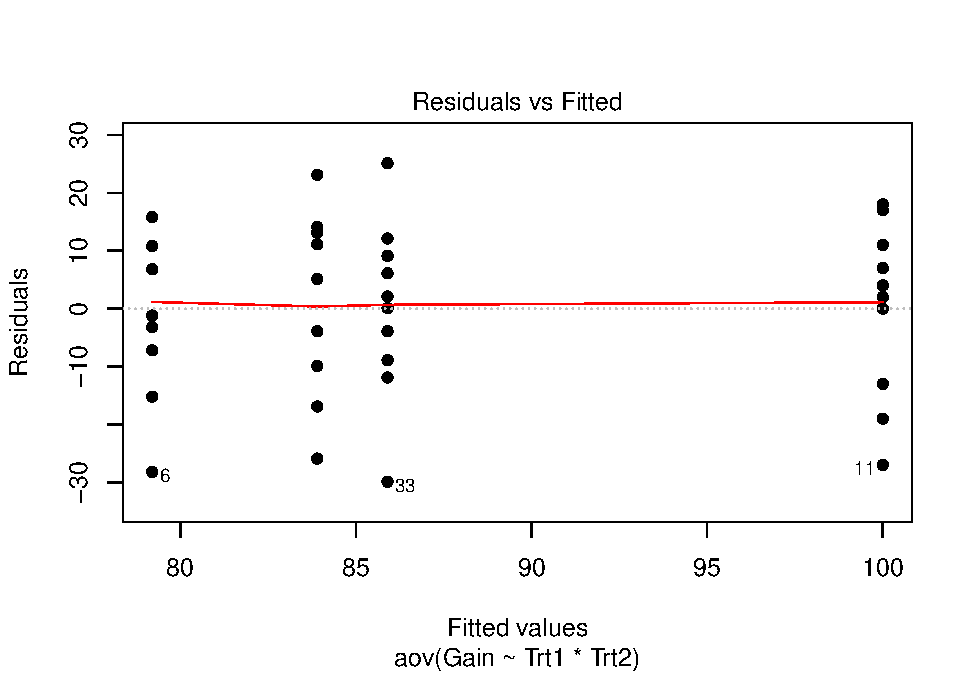
\includegraphics[width=0.25\linewidth]{svm-rmarkdown-article-example_files/figure-latex/unnamed-chunk-5-1}
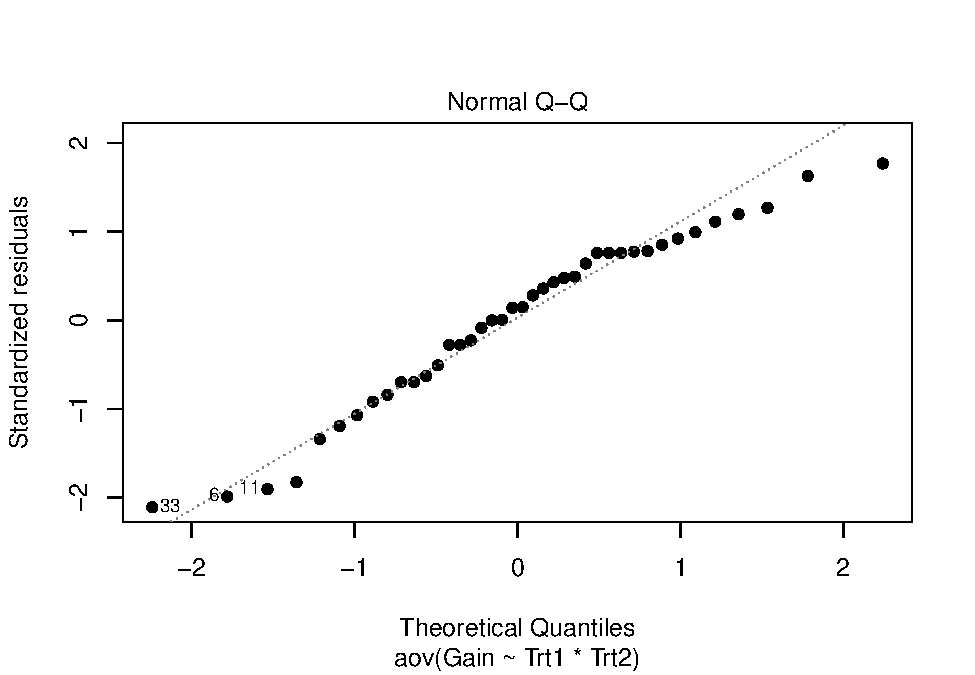
\includegraphics[width=0.25\linewidth]{svm-rmarkdown-article-example_files/figure-latex/unnamed-chunk-5-2}
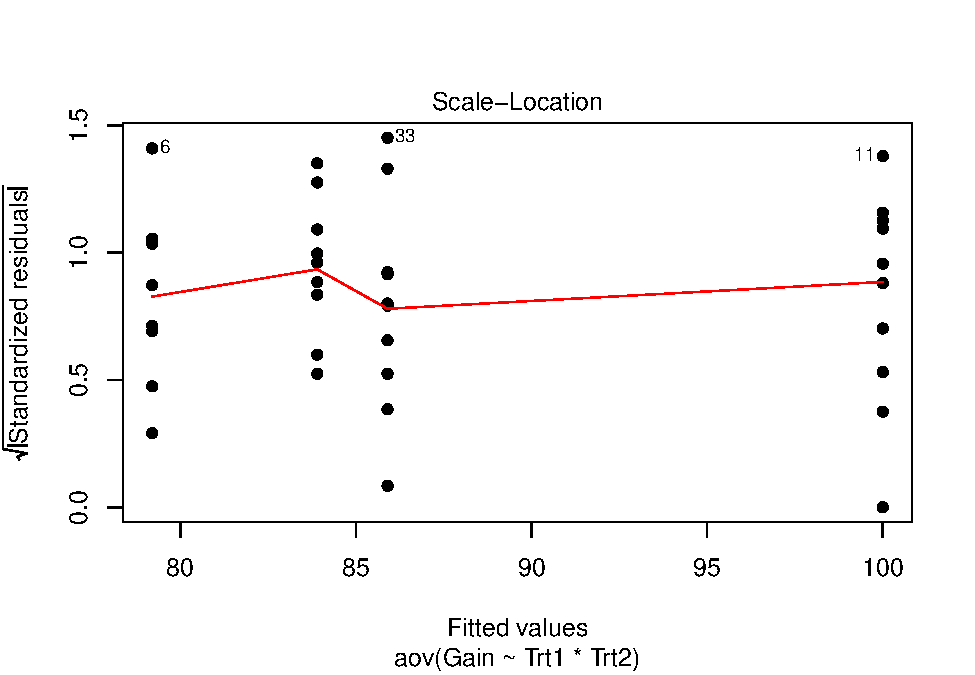
\includegraphics[width=0.25\linewidth]{svm-rmarkdown-article-example_files/figure-latex/unnamed-chunk-5-3}
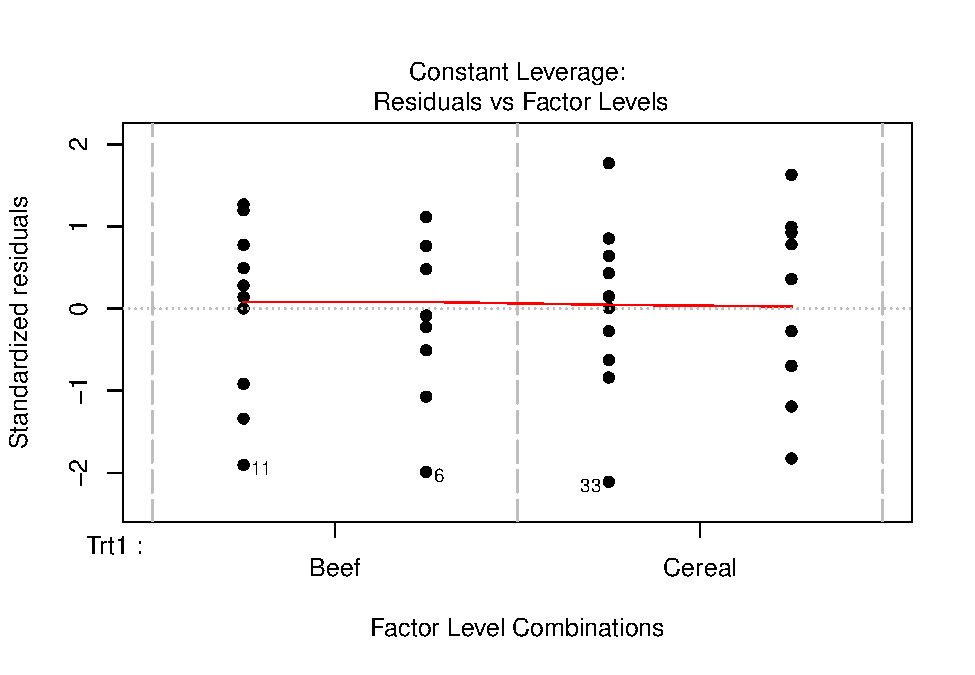
\includegraphics[width=0.25\linewidth]{svm-rmarkdown-article-example_files/figure-latex/unnamed-chunk-5-4}

\begin{enumerate}
\def\labelenumi{(\alph{enumi})}
\setcounter{enumi}{5}
\item
  \textcolor[rgb]{0.5,0.5,0.5}{Based on the residual plots, clearly explain whether assumptions in the model are satisfied or violated.}
\item
  \textcolor[rgb]{0.5,0.5,0.5}{Report the code here without output.}
\end{enumerate}

\begin{Shaded}
\begin{Highlighting}[]
\NormalTok{table_protein <-}\StringTok{ }\KeywordTok{read_excel}\NormalTok{(}\StringTok{"Protein.xlsx"}\NormalTok{)}
\KeywordTok{glimpse}\NormalTok{(table_protein)}
\CommentTok{# Install and load ggplot2 package before using ggplot function #}
\KeywordTok{ggplot}\NormalTok{(}\DataTypeTok{data =}\NormalTok{ table_protein, }\KeywordTok{aes}\NormalTok{(}\DataTypeTok{x =}\NormalTok{ Amount, }\DataTypeTok{y =}\NormalTok{ Gain, }\DataTypeTok{colour =}\NormalTok{ Source, }\DataTypeTok{group =}\NormalTok{ Source)) }\OperatorTok{+}\StringTok{ }
\StringTok{    }\KeywordTok{geom_point}\NormalTok{(}\KeywordTok{aes}\NormalTok{(}\DataTypeTok{shape =}\NormalTok{ Source, }\DataTypeTok{color =}\NormalTok{ Source), }\DataTypeTok{size =} \DecValTok{2}\NormalTok{) }\OperatorTok{+}\StringTok{ }\KeywordTok{labs}\NormalTok{(}\DataTypeTok{y =} \StringTok{"Weight Gained"}\NormalTok{, }
    \DataTypeTok{x =} \StringTok{"Amount of table_protein"}\NormalTok{, }\DataTypeTok{color =} \StringTok{"Source of table_protein"}\NormalTok{, }\DataTypeTok{shape =} \StringTok{"Source of table_protein"}\NormalTok{)}
\CommentTok{# Plots the Mean and 1SD error bars for each treatment group #}
\KeywordTok{ggplot}\NormalTok{(}\DataTypeTok{data =}\NormalTok{ table_protein, }\KeywordTok{aes}\NormalTok{(}\DataTypeTok{x =}\NormalTok{ Amount, }\DataTypeTok{y =}\NormalTok{ Gain, }\DataTypeTok{colour =}\NormalTok{ Source, }\DataTypeTok{shape =}\NormalTok{ Source, }
    \DataTypeTok{group =}\NormalTok{ Source)) }\OperatorTok{+}\StringTok{ }\KeywordTok{stat_summary}\NormalTok{() }\OperatorTok{+}\StringTok{ }\KeywordTok{labs}\NormalTok{(}\DataTypeTok{y =} \StringTok{"Weight Gained"}\NormalTok{, }\DataTypeTok{x =} \StringTok{"Amount of table_protein"}\NormalTok{, }
    \DataTypeTok{color =} \StringTok{"Source"}\NormalTok{, }\DataTypeTok{shape =} \StringTok{"Source"}\NormalTok{)}
\CommentTok{# Install and load ggpubr package before using ggline function #}
\KeywordTok{ggline}\NormalTok{(}\DataTypeTok{data =}\NormalTok{ table_protein, }\DataTypeTok{x =} \StringTok{"Amount"}\NormalTok{, }\DataTypeTok{y =} \StringTok{"Gain"}\NormalTok{, }\DataTypeTok{add =} \KeywordTok{c}\NormalTok{(}\StringTok{"mean"}\NormalTok{, }\StringTok{"jitter"}\NormalTok{), }
    \DataTypeTok{shape =} \StringTok{"Source"}\NormalTok{, }\DataTypeTok{color =} \StringTok{"Source"}\NormalTok{, }\DataTypeTok{linetype =} \StringTok{"Source"}\NormalTok{, }\DataTypeTok{ylab =} \StringTok{"Weight Gained"}\NormalTok{, }
    \DataTypeTok{xlab =} \StringTok{"Amount of table_protein"}\NormalTok{)}
\CommentTok{# Load mosaic package before using favstats function#}
\KeywordTok{favstats}\NormalTok{(Gain }\OperatorTok{~}\StringTok{ }\NormalTok{Source, }\DataTypeTok{data =}\NormalTok{ table_protein)}
\KeywordTok{favstats}\NormalTok{(Gain }\OperatorTok{~}\StringTok{ }\NormalTok{Amount, }\DataTypeTok{data =}\NormalTok{ table_protein)}
\KeywordTok{favstats}\NormalTok{(Gain }\OperatorTok{~}\StringTok{ }\NormalTok{Source }\OperatorTok{|}\StringTok{ }\NormalTok{Amount, }\DataTypeTok{data =}\NormalTok{ table_protein)}
\CommentTok{# favstats(Gain ~ Source+Amount, data=table_protein) Create Categorical}
\CommentTok{# variables so that plot of residuals versus each treatment combination can}
\CommentTok{# be obtained using plot function with the fitted model later #}
\NormalTok{table_protein}\OperatorTok{$}\NormalTok{Trt1 =}\StringTok{ }\KeywordTok{as.factor}\NormalTok{(table_protein}\OperatorTok{$}\NormalTok{Source)}
\NormalTok{table_protein}\OperatorTok{$}\NormalTok{Trt2 =}\StringTok{ }\KeywordTok{as.factor}\NormalTok{(table_protein}\OperatorTok{$}\NormalTok{Amount)}
\NormalTok{model_protein <-}\StringTok{ }\KeywordTok{aov}\NormalTok{(Gain }\OperatorTok{~}\StringTok{ }\NormalTok{Trt1 }\OperatorTok{*}\StringTok{ }\NormalTok{Trt2, }\DataTypeTok{data =}\NormalTok{ table_protein)}
\KeywordTok{summary}\NormalTok{(model_protein)}
\KeywordTok{pander}\NormalTok{(}\KeywordTok{summary}\NormalTok{(model_protein))}
\KeywordTok{sum}\NormalTok{((table_protein}\OperatorTok{$}\NormalTok{Gain }\OperatorTok{-}\StringTok{ }\KeywordTok{mean}\NormalTok{(table_protein}\OperatorTok{$}\NormalTok{Gain))}\OperatorTok{^}\DecValTok{2}\NormalTok{)}
\KeywordTok{plot}\NormalTok{(model_protein, }\DataTypeTok{pch =} \DecValTok{16}\NormalTok{)}
\CommentTok{# Pairwise comparisons using t tests with pooled Standard Deviation # The}
\CommentTok{# output gives a matrix of p values for each pair of treatments #}
\KeywordTok{pairwise.t.test}\NormalTok{(table_protein}\OperatorTok{$}\NormalTok{Gain, table_protein}\OperatorTok{$}\NormalTok{Trt2, }\DataTypeTok{p.adj =} \StringTok{"none"}\NormalTok{)}
\CommentTok{# Pairwise comparisons using t tests with pooled Standard Deviation and}
\CommentTok{# Bonferroni adjustment # The output gives a matrix of p values for each}
\CommentTok{# pair of treatments #}
\KeywordTok{pairwise.t.test}\NormalTok{(table_protein}\OperatorTok{$}\NormalTok{Gain, table_protein}\OperatorTok{$}\NormalTok{Trt2, }\DataTypeTok{p.adj =} \StringTok{"bonf"}\NormalTok{)}
\CommentTok{# Install and load the agricolae package before running the LSD.test}
\CommentTok{# function below # p.adj option in the LSD.test function can be used to}
\CommentTok{# apply different adjustments to control error rates#}
\KeywordTok{plot}\NormalTok{(}\KeywordTok{LSD.test}\NormalTok{(model_protein, }\DataTypeTok{trt =} \StringTok{"Trt2"}\NormalTok{, }\DataTypeTok{alpha =} \FloatTok{0.05}\NormalTok{))}
\NormalTok{(}\KeywordTok{LSD.test}\NormalTok{(model_protein, }\DataTypeTok{trt =} \StringTok{"Trt2"}\NormalTok{, }\DataTypeTok{alpha =} \FloatTok{0.05}\NormalTok{))}
\KeywordTok{pander}\NormalTok{(}\KeywordTok{TukeyHSD}\NormalTok{(model_protein, }\DataTypeTok{conf.level =} \FloatTok{0.95}\NormalTok{)[}\DecValTok{3}\NormalTok{])}
\KeywordTok{pander}\NormalTok{(}\KeywordTok{ScheffeTest}\NormalTok{(model_protein, }\DataTypeTok{conf.level =} \FloatTok{0.95}\NormalTok{)[}\DecValTok{3}\NormalTok{])}
\end{Highlighting}
\end{Shaded}




\newpage
\singlespacing 
\end{document}
